\section{SyzPass Design}
To overcome these shortcomings, we design SyzPass, a framework that comprehensively discovers primitives in vulnerabilities while automatically measuring and solving side effects residing in these primitives, generating actionable analyses to facilitate kernel exploit development. In this section, we illustrate the design of SyzPass, showing how it achieves automatic side effects solving.


\subsection{Workflow}

\begin{figure*}[htbp]
  \centering
  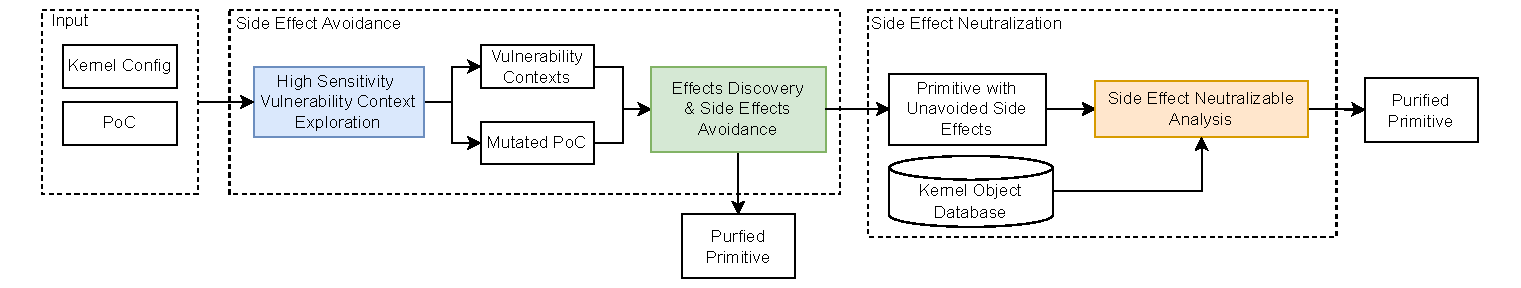
\includegraphics[width=0.99\linewidth]{figures/syzpass_pipeline.pdf}
  \caption{\label{fig:fuzz-graph}The workflow of SyzPass}
\end{figure*}

The workflow of SyzPass is shown in Figure~\ref{fig:fuzz-graph}. It takes as input the target kernel configuration and a PoC that triggers the vulnerability. The output is a set of primitives, each associated with a set of side-effect outcomes; a primitive may appear on a path that encounters zero or more side effects.
Furthermore, each side effect outcome is also tied to a corresponding strategy, including syscall sequences and sprayed data constraints for syscall avoidance, and kernel objects to neutralize residual side effects.

% primitives reside in the vulnerabilities and corresponding actionable side effects solving strategies consist of associated syscall sequence, data constraints for sprayed memory, and matched objects that can neutralize remaining side effects. 

Using the original PoC, SyzPass first explores vulnerability contexts to identify alternative syscall sequences that trigger the vulnerability, i.e., \emph{High Sensitivity Vulnerability Context Exploration}. It then explores execution paths after the initial corruption to search for alternative execution paths to avoid side effects, i.e., \emph{Primitive Discovery \& Side Effect Avoidance}.
For primitives where side effects are unavoidable, SyzPass examines memory layout requirements to neutralize them, i.e., \emph{Side Effect Neutralization Analysis}. Leveraging this analysis with a kernel heap object database that we collected, SyzPass matches suitable kernel objects to spray for neutralizing such unavoidable side effects.

% SyzPass first leverages high-sensitivity fuzzing to explore alternative vulnerability contexts the attacker can leverage. It then uses symbolic execution to analyze the possible execution paths that an attacker could manipulate the kernel to follow using memory spraying. Finally, it analyzes these paths and match associated data constraints with kernel memory objects to comprehensively apply  side effect avoidance and side effect neutralization to solve the side effects issue.


\subsection{High Sensitivity Vulnerability Context Exploration}
\label{sec:context_exploration}

The goal of the vulnerability context exploration component is to support syscall-adjustment-enabled avoidance. We leverage syscall fuzzing because it adjusts syscalls by design (e.g., sequence and argument values). On the other hand, it is significantly more difficult to fuzz attacker-sprayed memory, which is why we leave it to the next component.
%in exploring the vast search space of syscalls and arguments needed for context exploration. 

Prior work~\cite{lin2022grebe,zou2022syzscope,tan2023syzdirect,harbianqa,yome} employs fuzzing to explore targeted kernel areas. However, these approaches lack the sensitivity necessary to detect subtle changes in vulnerability contexts, as discussed in \S~\ref{other_tool_problem}. 

The primary reason is that most existing solutions are Syzkaller-based, retaining their original crash classification mechanism. However, the original mechanism determines that two crashes are the same if they share the identical initial corruption and bug-triggering function. While being effective for bug detection, this limits fuzzers' ability to identify subtle context changes behind the initial corruption, which can include additional effects, as illustrated in Figure~\ref{fig:motivating}. SyzScope makes a modification to this mechanism by identifying the first write-related corruption when the initial corruption is a read, and using it for crash classification. Unfortunately, it does not differentiate and record the various execution paths that may encounter different numbers or types of effects.
%\zhiyun{The description is not clear. Better use the motivating example to explain the subtle difference here.}

Therefore, we need to design an enhanced crash signature to enable more sensitive crash classification. Such an enhanced signature should distinguish seemingly identical crashes caused by different potential primitives and path constraints, while remaining efficient and robust. For such a mechanism, we propose three requirements: %\zhiyun{these requirements need to be explained with more details, e.g., examples. We can move pieces from later paragraphs here.}

\noindent\textbf{1. Sensitive:} It should be able to detect subtle context changes beyond the initial effect, which is critical for context exploration. For example, we should distinguish \circled{4}→\circled{5} from \circled{4}→\circled{6} in the motivating example (Figure~\ref{fig:motivating}).

\noindent\textbf{2. Noise Resilient:} One naive solution is to track post-initial-effect paths, which is the most sensitive.
However, this is susceptible to noise. Specifically, branches that are unrelated to the vulnerability may appear in the results. Additionally, branches associated with the vulnerability but unaffected by syscall arguments will also be included.
For example, the branches \circled{7}→\circled{8} and \circled{7}→\circled{9} would be differentiated under this approach, even though they are not influenced by the syscalls and should not factor into crash differentiation; instead, they should be differentiated by side effect avoidance by memory spraying (see \S\ref{sec:symbolic_execution}).

%While being sensitive, the mechanism must remain robust against noises, such as variables irrelevant to the vulnerability, memories influenced by heap spraying. This ensures the classification results remain stable.

\noindent\textbf{3. Efficient:} As classification is triggered on every crash and context exploration induces frequent failures, the classification mechanism must be lightweight. For example, if we were to track the influence of branches affected by syscalls (e.g., sequence and argument values), we would need to do so across the boundary of syscalls, due to dependencies among syscalls~\cite{dependency_measurement}. This can be prohibitively expensive, especially when conducted frequently. 
%tracing to identify whether a branch is influenced by syscall arguments or relevant to the vulnerability is highly unscalable, making it incompatible with our efficiency requirement. 
%\zhiyun{Efficiency of classification mechanism. Heavyweight due to cross-syscall tracing. That's why we have to resort to tracking symbolic memory instead of syscall arguments.}




%Due to our sensitivity requirement, our new mechanism must distinguish \circled{4}→\circled{5} from \circled{4}→\circled{6} in the motivating example. However, naively tracking all post-crash branches is susceptible to noise. Specifically, branches that are contextually related to the vulnerability may still appear in the results. Additionally, branches associated with the vulnerability but unaffected by syscall arguments are also included. For example, the branch at \circled{7} would be tracked under this approach, even though it is not influenced by the syscall sequence and should not factor into crash differentiation. Conversely, performing precise cross-syscall tracing to identify whether a branch is influenced by syscall arguments or relevant to the vulnerability is highly unscalable, making it incompatible with our efficiency requirement. 

To balance these requirements, we propose a lightweight branch set collection algorithm, as depicted in Algorithm~\ref{alg:effective-branchset}. Given a memory snapshot of the crashing kernel, the algorithm performs fast concolic execution to collect branches that are potentially influenced by syscall arguments.
%which serve as a complementary signature beyond the crash title.

% analyze every single crash, in order to differentiate crashes with new contexts. 
%It efficiently generates a set of context-relevant branches to facilitate crash differentiation.


\begin{algorithm}[htbp]
\caption{Efficient Branch Set Collection}
\label{alg:effective-branchset}
\begin{algorithmic}[1]
\Require Memory snapshot $S$
\Ensure  branch set $B$

\State $P \gets \emptyset$ \Comment{pending candidate branches}
\State $B \gets \emptyset$ \Comment{collected branch set}
\State $Bucket \gets \emptyset$ \Comment{map between IPDs and branches }
Symbolize(S)\Comment{symbolize UAF/OOB R memory }
% \State Symbolize heap-sprayed controllable memory in $S$

\While{execution continues}
    \State $rip \gets$ current instruction address

    \If{$rip \in \text{Bucket}$} \Comment{prune irrelevant branches}
        \State $P \gets P \setminus \text{Bucket}[rip]$
    \EndIf
    \If{$rip$ is a branch with unsymbolized condition}
        \State $(f, t) \gets$ jump from $rip$ to $target$
        \State $P \gets P \cup \{(f, t)\}$
        \State $ipd \gets \textsc{GetIPD}(f)$
        \State $\text{Bucket}[ipd] \gets \text{Bucket}[ipd] \cup \{(f, t)\}$
    \ElsIf{memory corruption operation is detected}
        \State $B \gets B \cup P$
        \State $P \gets \emptyset$
    \EndIf
\EndWhile

\State \Return $B$
\end{algorithmic}
\end{algorithm}

%Our key insight is that attacker influence on kernel execution primarily stems from two sources: memory spraying and bug-triggering syscall sequences. To avoid tracking the influence from syscalls, which is expensive due to the aforementioned cross-syscall challenge, we flip the problem by identifying branches \textit{affected} by memory spraying and avoiding using them to differentiate different crashes. 
Our key insight is that attackers mainly influence kernel execution through two channels: heap spraying and bug-triggering syscalls (including arguments). Because tracking syscall influence is expensive under cross-syscall interactions, we reverse the analysis: we detect spray-influenced branches and exclude them when distinguishing crash behaviors. This cuts overhead enough to run on every fuzzer-triggered crash.

Given that attackers mainly influence the execution (i.e., control flow) through two channels: syscalls and memory spraying, and the fact that tracking syscall influence is expensive (due to aforementioned cross-syscall interactions), our idea is to reverse the analysis.
Specifically, instead of identifying which branches are influenced by syscall arguments, we can identify spray-influenced branches and exclude them when distinguishing crash behaviors. This significantly reduces the analysis overhead, allowing this to be performed on every crash triggered by the fuzzer. 

To this end, we employ concolic execution by symbolizing UAF or OOB read memory. We detail the procedure in Algorithm~\ref{alg:effective-branchset}. As concolic execution progresses until the end of the syscall, we examine branches and their path constraints (if any) to extract the branch set.
If a path condition is not symbolized, i.e., not influenced by heap spraying memory (so that thus potentially influenced by bug-triggering syscall arguments), we add the corresponding branch into pending candidate branches \textit{P}, indicating that they are candidate branches for collection.

% The reason why these candidate branches are not directly merged into the final branch set \textit{B} is that we need an extra filter to exclude branches irrelevant to memory effects within this vulnerability.  
To exclude noise, we add candidate branches to the final set only when they are relevant to subsequent memory effects. We use the following heuristic: a branch is relevant iff at least one effect is control-dependent on it. Specifically, we apply \textit{immediate post-dominator} (IPD) analysis. The IPD of a branch is the first basic block guaranteed to execute regardless of branch direction; blocks after the IPD are not control-dependent on that branch. Therefore, if an effect occurs between the branch instruction and its IPD (i.e., it happens conditionally), we include it in the final branch set \textit{B}; otherwise, we treat it as noise and discard it.

% that are irrelevant to primitives beyond the initial crash\zhiyun{This sentence is difficult to parse. What is ``irrelevant to primitives'' and why ``beyond the initial crash''? I feel that we haven't given enough intuition about what we are trying to achieve here}. Thus, we apply \textit{immediate post-dominator} (IPD) analysis. The IPD of a branch is the first basic block that is guaranteed to execute after the branch, regardless of the direction taken. Thus, if memory corruption operations happen between a branch and IPD, the branch is considered to be potentially influential to it, and is merged to the final branch set \textit{B}; otherwise, the branch is treated as noise and ignored.

% This algorithm is efficient, as it yields results through concolic execution, and the computation of IPD is nearly linear.


% concolic execution by \textbf{symbolizing memory regions controllable via heap spraying}. During execution, branches with concrete (non-symbolic) conditions are considered unaffected by spraying, and are thus attributed to the syscall influence.


% While filtering out branches influenced by heap spraying helps reduce noise, it is not enough: many branches affected by syscall behavior may still be unrelated to the actual memory corruption. To more precisely isolate the control-flow decisions that are semantically relevant to the vulnerability, we apply \textit{immediate post-dominator} (IPD) analysis. The IPD of a branch is the first basic block that is guaranteed to execute after the branch, regardless of the direction taken.
% Our intuition is as follows: if execution reaches the IPD and no effects are triggered, then we say the branches taken did not contribute to the bug.



%While filtering out heap-spray-influenced branches already reduces noise, this alone is insufficient. Many syscall-influenced branches may still not contribute to the actual memory corruption. To further isolate only the branches that are semantically relevant to the vulnerability, we apply \textit{immediate post-dominator} (IPD) analysis. An IPD of a branch is the first instruction that always executes after the branch, regardless of which path is taken. Intuitively, if execution reaches the IPD without triggering memory corruption (e.g., UAF write), we conservatively discard the corresponding branch, since it does not influence whether the bug manifests. This enables precise pruning of irrelevant branches without relying on heavyweight dependency tracking.

With this new signature and fuzzing through mutation on the original PoC, we can effectively discover alternative syscall sequences for bug triggering, exploring vulnerability contexts in a highly sensitive manner, and setting foundations for subsequent analysis. 

\subsection{Effect Discovery and Side Effect Avoidance}
\label{sec:symbolic_execution}

\begin{figure}[htbp]
  \centering
  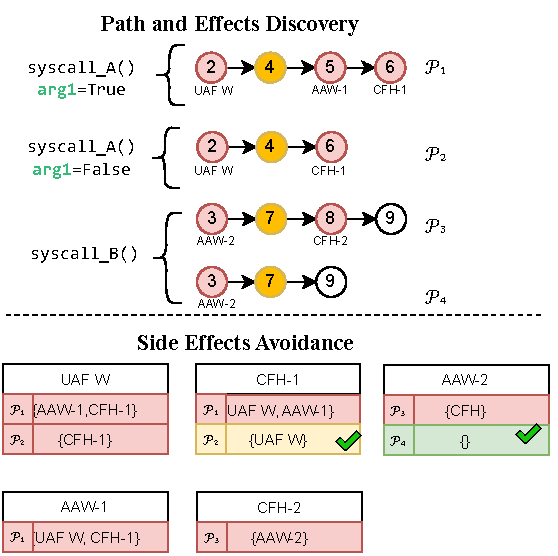
\includegraphics[width=\linewidth,trim=0 0 0 5, clip]{figures/symexec.pdf}
  \caption{\label{fig:symexec}Effects Discovery and Side Effect Avoidance}
\end{figure}

While the previous component explores various execution paths influenced by one source of attacker-controlled input, i.e., syscalls, this component focuses on paths affected by the other major input source: the attacker's sprayed memory.
In particular, this component employs symbolic execution by modeling the attacker's control over heap memory symbolically and analyzing potential memory effects and paths behind the initial corruption. 

Through symbolic execution, we perform fine-grained memory operation analysis to identify memory effects.
For example, if a \texttt{call} instruction targets a register containing symbolic data, we classify it as a control-flow hijack (CFH) effect.
Moreover, it also enables the exploration of alternative execution paths corresponding to each identified memory effect. Consequently, we can enumerate potential paths for each memory effect and perform side effect avoidance.

% This is crucial because additional effects may be discovered after the initial memory error, which has both positive and negative implications. On the one hand, more effects provide greater flexibility for primitive selection. On the other hand, observing multiple effects along a single execution path raises concerns about side effects. Knowing the complete set of effects associated with each path helps with side effect avoidance.

% Furthermore, along each symbolic execution path, we perform precise memory operation analysis leveraging the symbolic executor to identify potential effects. For example, if a \texttt{call} instruction targets a register containing symbolic data, we consider this a control-flow hijack (CFH) effect.

We illustrate this process through the motivating example in Figure~\ref{fig:symexec}. The upper part illustrates the paths and memory effects achievable through symbolic execution. The lower part summarizes, for each path, the set of associated effects. The red cells mark unresolved lethal side effects; yellow cells mark unresolved non-lethal side effects; green cells indicate no additional side effects on the path.


The symbolic execution starts with three vulnerability contexts (two \texttt{syscall\_A} related and one \texttt{syscall\_B} related) generated using the approach described in \S\ref{sec:context_exploration}. Notably, for \texttt{syscall\_B}, two paths $\mathcal{P}_3$ and $\mathcal{P}_4$ are discovered through symbolic execution.


% We assume the previous part context exploration component is finished with three PoCs generated (two \texttt{syscall\_A} related and one \texttt{syscall\_B} related). The advantage of using symbolic execution, for the PoC with \texttt{syscall\_B}, is that we can find both paths of  $\mathcal{P}_3$ and $\mathcal{P}_4$, not just one of them. This provides us more paths available and potentially more strategies for avoiding side effects.

% different potential paths of the motivating example vulnerability's different paths, as depicted in Figure~\ref{fig:symexec}. We start from 3 PoCs generated by the context exploration component. Suppose without heap spraying, their execution trajectory corresponds to $\mathcal{P}_1$ to $\mathcal{P}_3$. Using symbolic execution by symbolizing the attacker-sprayed memory, we find that it is possible to avoid the CFH effect, leading to $\mathcal{P}_4$.
%Finally, it is important that we record a set of execution paths (i.e., $\mathcal{P}_1$ to  $\mathcal{P}_4$) and the primitives associated with them.

% The second step is performing side effects avoidance. For analyze each potential primitive's associated paths, identifying those with minimal side effects to achieve side effects avoidance. For instance, for the AAW primitive, there are three paths $\mathcal{P}_1$,$\mathcal{P}_2$,$\mathcal{P}_3$ associated to it.  Since both $\mathcal{P}_1$,$\mathcal{P}_2$ contain pointer dereference related side effects, they then regarded fail to avoid side effects. Meanwhile $\mathcal{P}_3$ doesn't contain any side effects, so $\mathcal{P}_3$ is picked as the suitable path for the AAW primitive.

With these paths and associated effects mapped out, we can start triaging them and deciding on what effect(s) to choose as primitives. Ideally, for each potential primitive, we should pick a path with minimal side effects, as depicted in the lower half of Figure~\ref{fig:symexec}. In this example, if an attacker hopes to pick an AAW primitive, there are two options: AAW-1 from \texttt{syscall\_A()} and AAW-2 from \texttt{syscall\_B()}. The former has only one associated path: $\mathcal{P}_1$, and there are unfortunately two side effects, including a CFH. The latter has two associated paths $\mathcal{P}_3$ and $\mathcal{P}_4$, and $\mathcal{P}_4$ is completely free of side effects. Thus, $\mathcal{P}_4$ is the preferred choice for further exploit construction.

Similarly, if the attacker aims to select a CFH primitive, both syscalls offer viable options. However, CFH-1 associated with $\mathcal{P}_2$ (under \texttt{syscall\_A()}) would be the preferred choice, as its only associated side effect is a UAF write, which may not result in a crash and is therefore less likely to interfere with the exploit.
%In contrast, $\mathcal{P}_3$ contains no side effects and is therefore selected as the preferred path for this primitive. Thus, during the exploit development, the attacker can pick the $\mathcal{P}_3$ path to exploit the bug through the AAW primitive.


% To accurately model kernel behavior in weird machine states (i.e., after initial memory corruption happen), we leverage symbolic execution. With symbolized heap memory, we reason about how heap manipulations steer execution along different paths, and we perform precise memory operation analysis along these paths to identify potential primitives. Finally, with paths explored and primitives discovered, we analyze each potential primitive's associated paths, identifying those with minimal side effects to achieve side effects avoidance. We detail our key designs as follows.
Below, we describe the design of this component in more detail:

\noindent\textbf{1. Path Exploration:} For each vulnerability context associated with a PoC, we rerun the PoC to trigger the crash and take a kernel memory snapshot at the point of initial memory corruption. Using this snapshot, we symbolize the controllable heap-sprayed memory and initiate symbolic execution to explore subsequent execution paths. 

Unlike prior work, our analysis requires symbolic execution to reach the end of the bug-triggering syscall or interrupt handler. This is because we need to confirm the absence of side effects both \textit{before} triggering the primitive and \textit{after}. Thus, a complete execution path is required to expose all side effects associated with each primitive.

However, it can be expensive to explore every path till the end. To mitigate the scalability challenge, we design a pruning strategy based on how promising a path is, i.e., side-effect-free. In particular, we terminate symbolic states early when a memory access involves more than two levels of dereferences over symbolic pointers, e.g., \texttt{*(p->f->dp)} where p is a symbolic pointer. Deep pointer chains are unlikely to be satisfied by heap spraying in real-world attacks, making the corresponding paths ineffective (or at leat undesirable) for side-effect-free exploitation. %Therefore, such states can be safely pruned without compromising our analysis goals.

% In support of this strategy, we modify existing work's \cite{zou2022syzscope} memory model and customize for dereference depth tracking on symbolic pointers. detailed in Algorithm~\ref{alg:deref-depth}. During initialization, symbolic variables mapped to heap-sprayed memory are initialized with depth zero and marked.

In support of this strategy, we modify the existing work's \cite{zou2022syzscope} memory model and customize it for dereference depth tracking on symbolic pointers, detailed in Algorithm~\ref{alg:deref-depth}. Each symbolic variable from the heap-sprayed region is initialized with depth 0. When memory is accessed through a symbolic, unconstrained address, we assign a new symbolic variable to represent the pointer to the address, setting its depth to one plus the maximum depth among variables in the address expression. We then constrain this new variable to a dedicated dummy region to prevent repeated expansion.


% During initialization, symbolic variables mapped to heap-sprayed memory are initialized with depth zero. When a symbolic address points to previously unmarked memory, we create a new symbolic variable for that region and assign it a depth equal to the maximum depth among all symbolic variables in the address expression, plus one. This process is detailed in Algorithm~\ref{alg:deref-depth}.

\begin{algorithm}[htbp]
\caption{Dereference Depth Tracking}
\label{alg:deref-depth}
\begin{algorithmic}[1]
\Require Snapshot $S$, symbolic region $R$
\Ensure Depth map $D$ for symbolic variables

\State Initialize depth map $D$ bound to state
\ForAll{$a \in R$}
    \State $v \gets \textsc{SymbolicVar}(a)$,\quad $D[v] \gets 0$
\EndFor

\While{execution continues}
    \If{accessed address $e$ is symbolic and unconstrained}
        \State $v \gets \textsc{SymbolicVar}(e)$
        \State $D[v] \gets \max\{ D[u] \mid u \in \textsc{Vars}(e) \} + 1$
        \State Constrain $v$ to dummy region
    \EndIf
\EndWhile
\end{algorithmic}
\end{algorithm}



% \begin{algorithm}[H]
% \caption{Pointer Dereference Depth Tracking}
% \label{alg:deref-depth}
% \begin{algorithmic}[1]
% \Require Symbolic state $s$, heap spray region $H$
% \Ensure Per-State Mapping $D$ from symbolic variables to depth

% \State $D \gets \emptyset$
% \ForAll{$a \in H$}
%     \State $D[\textsc{Sym}(a)] \gets 0$
% \EndFor

% \While{symbolic execution continues}
%     \If{access $e$ is symbolic and $e \rightarrow m$ is unmarked}
%         \State $v \gets \textsc{Sym}(m)$
%         \State $D[v] \gets \max\{ D[u] \mid u \in \textsc{Vars}(e) \} + 1$
%         \State Mark $m$
%     \EndIf
% \EndWhile
% \end{algorithmic}
% \end{algorithm}




\noindent\textbf{2. Primitive Discovery:} During symbolic execution, we inspect each memory operation to identify exploit primitives, following the definitions in prior work~\cite{zou2022syzscope}.
For every memory write, we classify primitives based on the target address and value: writes to symbolic addresses are categorized as Arbitrary Address Write (AAW) or Constrained Address Write (CAW); writes targeting heap-sprayed memory are denoted as OOB/UAF Write (OUW); writes with symbolic values are classified as Arbitrary Value Write (AVW) or Constrained Value Write (CVW). The arbitrariness of addresses and values is determined via SMT solving over the collected symbolic constraints.
In addition, we monitor function call targets and arguments to detect Invalid Free (IF) and Control Flow Hijack (CFH).
We exclude memory read operations from primitive collection, as they do not directly enable privilege escalation, though their access patterns and pointer dereferences are still tracked as side effects. 
%\zhiyun{I thought we consider only pointer dereferences as side effects?}

\noindent\textbf{3. Side Effect Avoidance:} With the collected paths and primitives, we devise strategies to avoid side effects by selecting, for each primitive, the execution path with minimal side effects, ideally no side effects.

A prerequisite for this comparison is to identify all execution paths corresponding to the same primitive. To achieve this, we establish a mechanism to associate instances of the same primitive across different paths by labeling them based on their type and the instruction address at which they occur. This is simple yet effective, and it supports comparing primitives across different vulnerability contexts.
%ensuring that semantically equivalent primitives are treated uniformly during analysis.

Once all paths associated with a given primitive are identified, we compute a side effect set for each path. Since we define side effects as all observable effects excluding a selected primitive itself, we construct each side effect set by subtracting the primitive
%and its corresponding pointer dereference constraints\zhiyun{what is the constraints here? did we introduce it before?} 
from the path's overall effect set. These side effect sets serve as the basis for comparison and selection, e.g., we can rank primitives based on the minimum number of associated side effects.

As discussed in \S~\ref{chap:eps}, pointer dereferences related side effects are particularly critical, as they lead to kernel crashes if mishandled. Thus, such side effects must be avoided or neutralized. Otherwise, a primitive associated with such side effects is considered unusable. In the next section, we discuss solutions to neutralize such side effects, if they cannot be avoided, e.g., all paths associated with a primitive incur such side effects.
%first de-prioritize any path whose side effect set includes such high-risk operations.

%We then analyze the generated sets to identify paths and rank order them according to the number of side effects, i.e., zero being the best. 
%As discussed in Section~\ref{chap:eps}, pointer dereferences related side effects are particularly critical, as they lead to kernel crashes if mishandled. Thus, we first de-prioritize any path whose side effect set includes such high-risk operations.
%\zhiyun{again, we need to be clear whether we consider only pointer dereferences as side effects.} 
%Among the remaining candidates, we select the path with the fewest residual side effects as the preferred execution strategy. 

%Through this process, we systematically leverage the explored vulnerability contexts and post-corruption execution paths to discover primitives and avoid side effects. In some cases, however, we may still want to consider primitives associated with non-ideal paths, i.e., those that exhibit pointer dereference-related side effects and are inherently unavoidable. For example, it is possible that all paths have the same kind of side effect for a particular primitive. To address these cases, we leverage side-effect neutralization technique, which we detail next.

\subsection{Side Effects Neutralization Analysis}
SyzPass performs neutralization with primitive-aware site reasoning. For a selected primitive site $s$, we separately determine whether $s$ is preserved as a useful primitive and whether there exists a path where all residual effects can be avoided by path selection or neutralized after they occur. This separation matters because a pointer-related primitive can be useful once its pointer target is attacker-controlled, while a value-write or bounded-write primitive must corrupt a useful victim-object field rather than attacker-controlled payload data.

SyzPass separates this reasoning from the attacker's capability model. In the baseline model, the attacker can trigger the bug from an unprivileged context, control syscall arguments and heap-sprayed data, and reclaim vulnerable memory with sprayable kernel objects, but cannot directly manufacture arbitrary valid kernel pointers. The pointer-materialization model ($\mathsf{PM}$) additionally assumes address disclosure and kernel-addressable attacker-controlled memory. Recent exploitation techniques motivate this stronger model: software side channels can disclose kernel addresses from unprivileged contexts~\cite{kernelsnitch}, and recent KernelCTF writeups show that attackers can place fake kernel-resident payloads at known kernel addresses with techniques such as NPerm~\cite{kernelctf-nperm}. Fixed or weakly randomized kernel regions have also appeared in real systems, as illustrated by the \texttt{cpu\_entry\_area} randomization issue and its use in exploit construction~\cite{cve20230597,kernelctf-cpuentry}. These techniques make pointer materialization realistic in many environments. Still, SyzPass retains object matching because such techniques can be unavailable in emulated environments such as QEMU TCG, may depend on deployment-specific side channels, and may be partially mitigated in future kernels. Object matching therefore remains a more portable fallback when a real sprayed object can satisfy the side effect.

Formally, let $\mathcal{P}_s$ be the explored paths that reach primitive site $s$, $E(p)$ be the memory effects on path $p$, and $C_p$ be the path constraints. SyzPass accepts site $s$ under capability model $\kappa$ iff there exists a path that preserves the selected site and makes every residual effect safe:
\[
\begin{aligned}
\mathsf{Accept}_{\kappa}(s) \triangleq
\exists p \in \mathcal{P}_s.\;
\mathsf{Preserve}_{\tau(s)}(s,C_p) \land {}\\
\forall e \in E(p)\setminus\{s\}.\ \mathsf{Safe}_{\kappa}(e,C_p).
\end{aligned}
\]
This outer existential captures side-effect avoidance: if one explored path reaches the same primitive site without a dangerous residual effect, SyzPass chooses that path instead of neutralizing the effect. For residual effects that remain on the chosen path, SyzPass uses the same safety predicate across primitive types:
\[
\begin{aligned}
\mathsf{Safe}_{\kappa}(e,C_p) \triangleq
\mathsf{OM}(e,C_p) \lor {}\\
(\kappa=\mathsf{PM} \land \mathsf{Ptr}(e) \land \mathsf{Mat}(e,C_p)).
\end{aligned}
\]
Here, $\mathsf{OM}$ denotes object matching against a sprayable object layout, $\mathsf{Ptr}(e)$ holds for pointer-shaped residual effects, and $\mathsf{Mat}$ denotes satisfying such a pointer-shaped effect under $\mathsf{PM}$. The primitive-specific part is $\mathsf{Preserve}$, summarized in Table~\ref{tab:primitive-aware-rules}. $\mathsf{Ctrl}(x)$ means that $x$ is attacker-controlled through the vulnerable object or sprayed data, $\mathsf{Sym}(x)$ means that $x$ remains symbolic in the path constraints, and $\mathsf{DFLike}$ denotes an invalid free whose argument is the vulnerable object itself or adjacent memory rather than an attacker-forged pointer. Let $\mathcal{F}_{u}$ be the set of meaningful victim-object fields, excluding attacker-controllable payload regions. For value writes, $\mathsf{field}(\mathsf{dst}(s))$ is the determined destination field on the analyzed path.

\begin{table}[t]
  \centering
  \small
  \renewcommand{\arraystretch}{1.08}
  \resizebox{\linewidth}{!}{%
  \begin{tabular}{ll}
    \toprule
    \textbf{Primitive type $\tau(s)$} & \textbf{$\mathsf{Preserve}_{\tau(s)}(s,C_p)$} \\
    \midrule
    CFH/FPD & $\mathsf{Ctrl}(\mathsf{target}(s))$ \\
    AAW & $\mathsf{Ctrl}(\mathsf{dst}(s))$ \\
    IF$_{sym}$ & $\mathsf{Sym}(\mathsf{arg}(s))$ \\
    IF$_{con}$ & $\mathsf{DFLike}(s)$ \\
    OUW/CAW & $\exists f \in \mathcal{F}_{u}.\ \mathsf{SAT}(C_p \land \mathsf{dst}(s) \in f)$ \\
    CVW/AVW & $\mathsf{Ctrl}(\mathsf{val}(s)) \land \mathsf{field}(\mathsf{dst}(s)) \in \mathcal{F}_{u}$ \\
    \bottomrule
  \end{tabular}}
  \caption{Primitive-specific preservation predicates. $\mathsf{Ctrl}$ means attacker-controlled, $\mathsf{Sym}$ means symbolic, and $\mathsf{DFLike}$ denotes double-free-like invalid free.}
  \label{tab:primitive-aware-rules}
\end{table}

For the object-matching backend, our design converts the side effects associated with a path into a \emph{required} memory layout, and each candidate object into an \emph{object} memory layout. We then compare the two and determine whether it is a match. If so, the side effect can be neutralized by spraying the corresponding object.
%By leveraging the memory layout of these objects, side effects can be neutralized during execution. We convert each path's data constraints\zhiyun{what kind of constraints?} and pointer-dereference relationships and kernel objects into a unified memory layout representation for effective comparison. 
We detail our design below, starting with a unified memory layout representation to support the matching:

\noindent\textbf{1. Memory Layout Representation Design:} We design our memory layout representation as a nested structure, depicted in Figure~\ref{fig:memlayout}.

\begin{figure}[htbp]
  \centering
  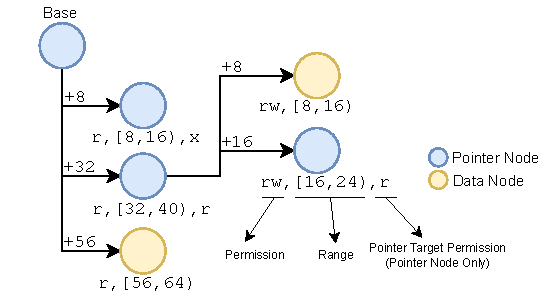
\includegraphics[width=\linewidth,trim=0 0 0 0, clip]{figures/memlayout.pdf}
  \caption{\label{fig:memlayout}Unified Memory Layout Representation}
\end{figure}

%\zhiyun{add a simple code example like if (valmem[56] $>$ 10) and explain how this is turned into a data node.}


In this representation, the memory layout is modeled as a tree, where each node represents a memory region (e.g., a field of an object). Each node is annotated with a byte range \([lo, hi)\), indicating the region's offset within the object, and an access permission field denoting the required memory access permissions.

Nodes are divided into two types. \textit{Pointer nodes} (blue) may point to another memory region in the layout and are annotated with an additional field: the target permission, which specifies the required permission of the pointee. This field allows us to simplify the tree by omitting the actual child nodes of the pointer when appropriate. Pointer nodes can have children, enabling the tree to recursively encode nested pointer relationships. The root node always represents a pointer to the kernel object (e.g., freed or accessed out-of-bounds) or the sprayed heap memory. Using the example in Figure~\ref{fig:memlayout}, we see the object associated with the root node has two pointer fields at two different offsets, i.e., 8 and 32, respectively. Furthermore, the object the second pointer points to has a pointer as well at offset 16.

\textit{Data nodes} (yellow) represent plain memory regions and are always leaf nodes in the tree. For these nodes, the byte range has special meanings. From the required memory layout side, the range indicates the memory whose values have to be specific. This is because of path constraints collected during symbolic execution. For example, there can be a conditional statement, such as \texttt{if(vulmem[56:64] > 10)}, whose true branch is taken in a path (e.g., to reach a particular effect). This results in the creation of a data node occupying the memory range [56, 64) within the required layout, as illustrated in Figure~\ref{fig:memlayout}. From the object memory layout side, a similar data node can be created if we know the corresponding memory value is controllable by an attacker, e.g., a buffer that can be initialized via syscall arguments.

Under this design, we can model nested pointer dereference chains to achieve object pairing. Furthermore, the concept of data nodes enables us to satisfy data requirements matching as well. These are the two most critical matching criteria we have observed in practice.

Lastly, there is a size annotation of the tree (not shown in the figure), indicating the total size of the kernel object or the sprayed heap memory. This size can provide a hint about which SLUB cache the vulnerable object belongs to, which will be helpful for object pairing. 


%pairing memory regions requiring constraints with controllable parts of spraying objects, increasing the practicality of matching.

\noindent\textbf{2. Required Memory Layout Construction:} For each path containing one or more side effects (pointer dereference), we construct a required memory layout using a three-phase process depicted in Figure~\ref{fig:memlayout_path}.


\begin{figure*}[htbp]
  \centering
  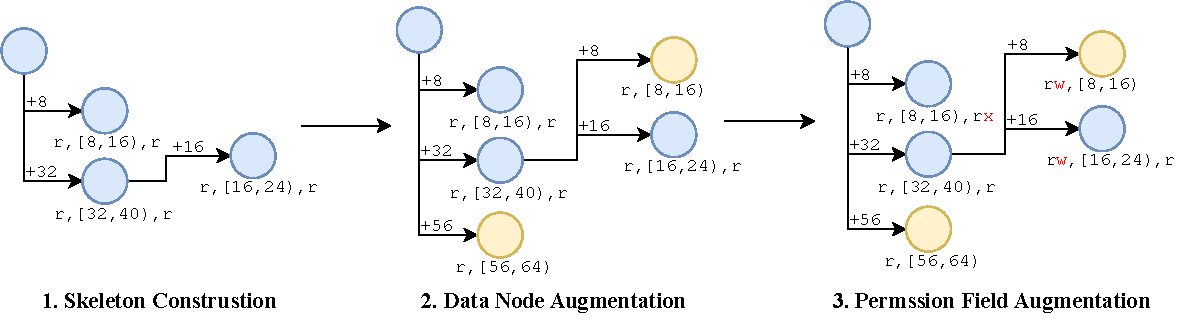
\includegraphics[width=0.9\linewidth,trim=0 5 0 0, clip]{figures/path_layout_creation.pdf}
  \caption{\label{fig:memlayout_path}Memory Layout Construction for Execution Path}
\end{figure*}

We initialize the tree and annotate the vulnerable object size information extracted from the KASAN report. Using this layout tree, we start the first phase, skeleton construction, where we capture pointer dereference relationships and initialize the tree. We iterate over symbolic pointer creations to identify newly introduced symbolic pointers and their corresponding base pointers, whose values are used to compute the new addresses. The relative offset is obtained by evaluating the difference between the new pointer's address and the base pointer's value using the symbolic solver. With the offset, we can generate the range needed for the attribute of the node. 
%For heap-spraying controllable memory, we designate its base pointer as the root node of the layout tree and calculate the offset by subtracting its address from the boundary of the sprayed memory region. Each such pair is added to the layout tree as a pointer edge, with default permissions initialized to read. 

Next, we traverse the remaining data constraints to augment the layout with data nodes. For each constraint, we identify the pointer used to access the memory region, compute the offset from the pointer’s base value to the target address using the solver, and determine the accessed byte range based on the data size of the related symbolic variables. A corresponding data node is then added as a child of the pointer node in the layout tree.

Finally, we parse the memory effects list of the path, augment write and execute permission among the layout tree based on the effect type and recorded constraint values.

Note that, as an optimization, we can first construct a tree for all effects on a path. Then, depending on the primitive picked, its corresponding nodes can be removed. 
%To further modify the layout for the need of the primitive, we trim the tree to exclude the current primitive from it, leaving it not used for comparison and neutralization. For a typical pointer dereference-related primitive, we achieve this by deleting the corresponding node and their children among the tree. 




\noindent\textbf{3. Memory Layout Reconstruction for Objects:} We collect objects among existing object databases from prior work to achieve memory layout reconstruction \cite{chen2019slake,chen2020systematic,wang2023alphaexp}, and assume them as sprayable and exploitable. To pair these objects with a required memory 
layout, we develop a simple algorithm to construct the object memory layout information through statically analyzing the kernel. In short, we parse the layout information of each structure to pinpoint pointers, then we iteratively generate the layout for pointers to model the pointer-dereference relationship. 

Following prior analysis of attacker-controllable fields in kernel objects~\cite{chen2020systematic}, we enrich object layouts with data nodes to represent memory regions that are considered user-controllable. In this context, a data node denotes an object field whose content can be influenced by the attacker. 


\noindent\textbf{4. Object Pairing for Side Effects Neutralization:} Our object pairing process consists of two phases. The first mode performs strict matching, requiring both data nodes and pointer dereference chains to match for precise analysis. However, if data node matching fails, it is also reasonable to consider a relaxed mode that only considers the pointer dereference structure for approximate matching. This is also useful since the exploit developer can perform manual analysis to understand whether the data constraints can be satisfied without requiring attacker-controllable memory specifically. For instance, if the data constraint requires some part of the vulnerable memory to be greater than or equal to zero, it is likely satisfiable by many objects naturally. We leave more precise data constraint solving as future work.

In both modes, we trim the primitive from associated path layouts to prevent the matching to neutralize the primitive, ensuring its exploitability. Then we match path layouts with object layouts one by one. Specifically, we check whether the required layout can align with the object layout without violating structural or permission constraints. For each pointer node in the path layout, we search for a matching node in the object layout that (i) covers an equal or greater byte range, (ii) provides equal or greater permission.
%\zhiyun{I don't understand what we mean by ``preserving the relationship''}
If a matching node is found, we recursively compare its children, following the pointer chain. In strict mode, we also require data nodes in the path to be matched precisely by data nodes in the object. 
%In relaxed mode, data nodes are ignored, allowing broader but potentially less precise matches.

A successful match means all pointer dereference side effects in the symbolic execution path can be safely neutralized using the object's memory layout. This lets the exploit generation continue without causing access violations or corrupting other kernel data. In such cases, we consider the neutralization successful and include the corresponding primitive, path, and matched object in our final output.
